\section*{Lecture 10}

\subsection*{1.} A door system with damping can, to some extent, be modelled by a mass spring system with damping. We assume that the door system is described by $y(t)$ and modelled by a mass spring system with critical damping. The function $y$ describes how much the door is open with $y(t) = 0$ for the door being closed.

\subsubsection*{a.} Express the constants $c_1$ and $c_2$ in the general solution
\[ 
y(t) = e^{- \alpha t} \left( c_1 + c_2t \right)
\]
for a mass spring system with critical damping in terms of the initial values $y(0) = K_0$ and $y'(0) = K_1$. 
\bigbreak
We calculate the derivative of the general solution as
\[ 
y'(t) = e^{-\alpha t} \left( c_2 (1 - \alpha t) - \alpha c_1 \right)
.\]
We therefore get the two equations
\begin{align*}
  e^{0} \left( c_1 + 0 \right) &= K_0 \\
  e^{0} \left( c_2 \left( 1 - 0 \right) - \alpha c_1 \right) &= K_1 \\
.\end{align*}
The first equation gives $c_1 = K_0$ and this can be inserted into the second equation as
\begin{align*}
  c_2 - \alpha K_0 &= K_1 \\
  c_2 &= K_1 + \alpha K_0
.\end{align*}
This gives the particular solution as
\[ 
  y(t) = e^{-\alpha t} \left( K_0 + (K_1 + \alpha K_0) t\right)
.\]


\subsubsection*{b.} Derive a condition on $K_0 > 0$ and $K_1$ such that there is a $t_0 > 0$ with $y(t_0) = 0$. Find $t_0$. Note that this scenario corresponds to slamming the door.
\bigbreak
We want the scenario $y(t_0) = 0$. This gives:
\begin{align*}
  y(t_0) &= 0 \\ 
  e^{-\alpha t_0} \left( K_0 + \left( K_1 + \alpha K_0 \right)t_0 \right) &= 0 \\
  K_0 + \left( K_1 + \alpha K_0 \right) t_0 &= 0 \\
  t_0 &= - \frac{K_0}{K_1 + \alpha K_0}
.\end{align*}
We already have $K_0 > 0$ but we also want $t_0 > 0$. This means $K_1 + \alpha K_0 < 0$. This gives
\[ 
\frac{K_1}{K_0} < -\alpha
.\]


\subsection*{2.} Consider the general solution of an undamped mass spring system
\[ 
y(t) = c_1 \cos \left( \omega_0 t \right) + c_2 \sin \left( \omega_0 t \right)
.\]

\begin{figure} [ht]
  \centering
  \caption{}
  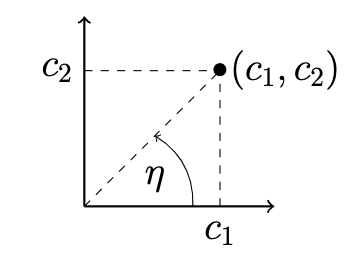
\includegraphics[width=0.35\linewidth]{../figures/f10_1.png}
  \label{fig:f10_1}
\end{figure}

\subsubsection*{a.} Express $c_1$ and $c_2$ in therms of
\[ 
A = \sqrt{c_1^2 + c_2^2}
\]
and the angle $\eta$ as depicted in \textbf{\autoref{fig:f10_1}}.
\bigbreak
From trigonometry we have
\begin{align*}
  c_1 &= A\cos \eta \\
  c_2 &= A\sin \eta
.\end{align*}



\subsubsection*{b.} Use the trigonometric identity
\[ 
\cos \left( a + b \right) = \cos a \cos b - \sin a \sin b
\]
to show that the general solution can be expressed as
\[ 
y(t) = A \cos \left( \omega_0 t - \eta \right), \tan \eta = \frac{c_2}{c_1}
.\]
\bigbreak
We have the general solution
\[ 
y(t) = c_1 \cos \left( \omega_0 t \right) + c_2 \sin \left( \omega_0 t \right)
.\]
Which we want to rewrite with
\[ 
\cos \left( a + b \right) = \cos a \cos b - \sin a \sin b
.\]
As the wanted solution has $\eta$ in the argument of the cosine we will use $a = \omega_0 t$ and $b = \eta$. We therefore get
\[ 
\cos \left( \omega_0 t - \eta \right) = \cos (\omega_0 t) \cos\eta + \sin \left( \omega_0 t \right) \sin \eta
.\]
We now compare
\[ 
A \cos \left( \omega_0 t - \eta \right) = A \left( \cos \left( \omega_0 t \right) \cos\eta + \sin \left( \omega_0 t \right) \sin \eta \right)
\]
to
\[ 
c_1 \cos (\omega_0 t) + c_2 \sin (\omega_0 t)
.\]
We therefore get
\[ 
  c_1 = A \cos \eta \quad c_2 = A \sin \eta
.\]
We also have
\begin{equation*}
  \tan \eta = \frac{A \sin \eta}{A \cos \eta} = \frac{c_2}{c_1}
.\end{equation*}


\subsection*{3.} Follow the procedure of Exercise 2 to show that
\[ 
y(t) = A(t) \cos (\omega t - \eta), A(t) = e^{-\alpha t} \sqrt{c_1^2 + c_2^2}, \tan \eta = \frac{c_2}{c_1}
\]
is an alternative way to express the general solution
\[ 
y(t) = e^{-\alpha t} \left( c_1 \cos (\omega t) + c_2 \sin (\omega t) \right)
\]
of an underdamped mass spring system.
\bigbreak
From exercise 2 we know that
\[ 
c_1 \cos \left( \omega t \right) + c_2 \sin (\omega t) = \sqrt{c_1^2 + c_2^2} \cos(\omega t - \eta)
.\]
We can plug this into the expression as
\[ 
y(t) = e^{-\alpha t} \sqrt{c_1^2 + c_2^2} \cos \left( \omega t - \eta \right)
.\]
We now define
\[ 
A(t) = e^{-\alpha t} \sqrt{c_1^2 + c_2^2} \implies y(t) = A(t) \cos \left( \omega t - \eta \right)
.\]
And from before we also know that
\[ 
\tan \eta = \frac{c_2}{c_1}
.\]



\subsection*{4.} Solve the IVP
\[ 
x^2 y''(x) + 3xy'(x) = - y(x), x>0, y(2) = 0, y'(2) = 1
.\]
\bigbreak
We rewrite the IVP to the standard form for an Euler-Gauchy equation as
\[ 
x^2 y''(x) + 3xy'(x) + y(x) = 0, x>0
.\]
We compare this with the standard form
\[ 
x^2 y''(x) + axy'(x) + by(x) = 0
.\]
And see that $a = 3$ and $b = 1$ which gives
\[ 
(1-a)^2 = 4 = 4b
.\]
This is Case II which has the general solution
\[ 
y(x) = x^{\frac{1}{2} (1-a)} \left( c_1 + c_2 \ln x \right) = \frac{1}{x} \left( c_1 + c_2 \ln x \right)
.\]
This has the derivative
\[ 
  y'(x) = - \frac{1}{x^2} \left( c_1 + c_2 \ln x \right) + \frac{1}{x}c_2 \frac{1}{x} = - \frac{1}{x^2} \left( c_1 - c_2 + c_2 \ln x \right)
.\]
We have the initial values
\begin{align*}
  y(2) &= 0 \\
  \frac{1}{2} \left( c_1 + c_2 \ln 2 \right) &= 0 \\
  c_1 + c_2 \ln 2 &= 0 \\
  c_1 &= - c_2 \ln 2 \\
  y'(2) &= 1 \\
  - \frac{1}{4} \left( - c_2 \ln 2 - c_2 + c_2 \ln 2 \right) &= 1 \\
  -c_2 &= -4 \\
  c_2 &= 4 \\
  c_1 &= -4 \ln 2
.\end{align*}
This gives the particular solution
\[ 
y_p(x) = \frac{1}{x} \left( - 4 \ln 2 + 4 \ln x \right)
.\]

